\section{矩阵的特征值与特征向量}

\subsection{矩阵的特征值}

\begin{theorem}[特征多项式展开定理]
    设 $\vb*{A}$ 是 $n$ 阶矩阵,则 $\vb*{A}$ 的特征多项式为 
    $$f(\lambda)=|\lambda\vb*{E}-\vb*{A}|=\lambda^n-a_1\lambda^{n-1}+\cdots+(-1)^ka_k\lambda^{n-k}+\cdots+(-1)^na_n$$
    其中 $a_k$ 是 $\vb*{A}$ 的所有 $k$ 阶主子式之和,即 
    $$a_k=\sum_{1\leqslant j_1<\cdots<j_k\leqslant n}\mqty|a_{j_1j_1}&\cdots&a_{j_1j_k}\\\vdots&&\vdots\\a_{j_kj_1}&\cdots&a_{j_kj_k}|$$
    特别地 $a_1=\tr\vb*{A},~a_n=\det\vb*{A}.$
    对于常见的 3 阶矩阵有 $$f(\lambda)=\lambda^3-\tr\vb*{A}\cdot\lambda^2+\qty(\mqty|a_{11}&a_{12}\\a_{21}&a_{22}|+\mqty|a_{11}&a_{13}\\a_{31}&a_{32}|+\mqty|a_{22}&a_{23}\\a_{32}&a_{33}|)\lambda-\det\vb*{A}.$$
\end{theorem}

图 \ref{fig:kjiezzshi} 是 $a_2$ 的形象化表达.
\begin{figure}[H]
    \centering
    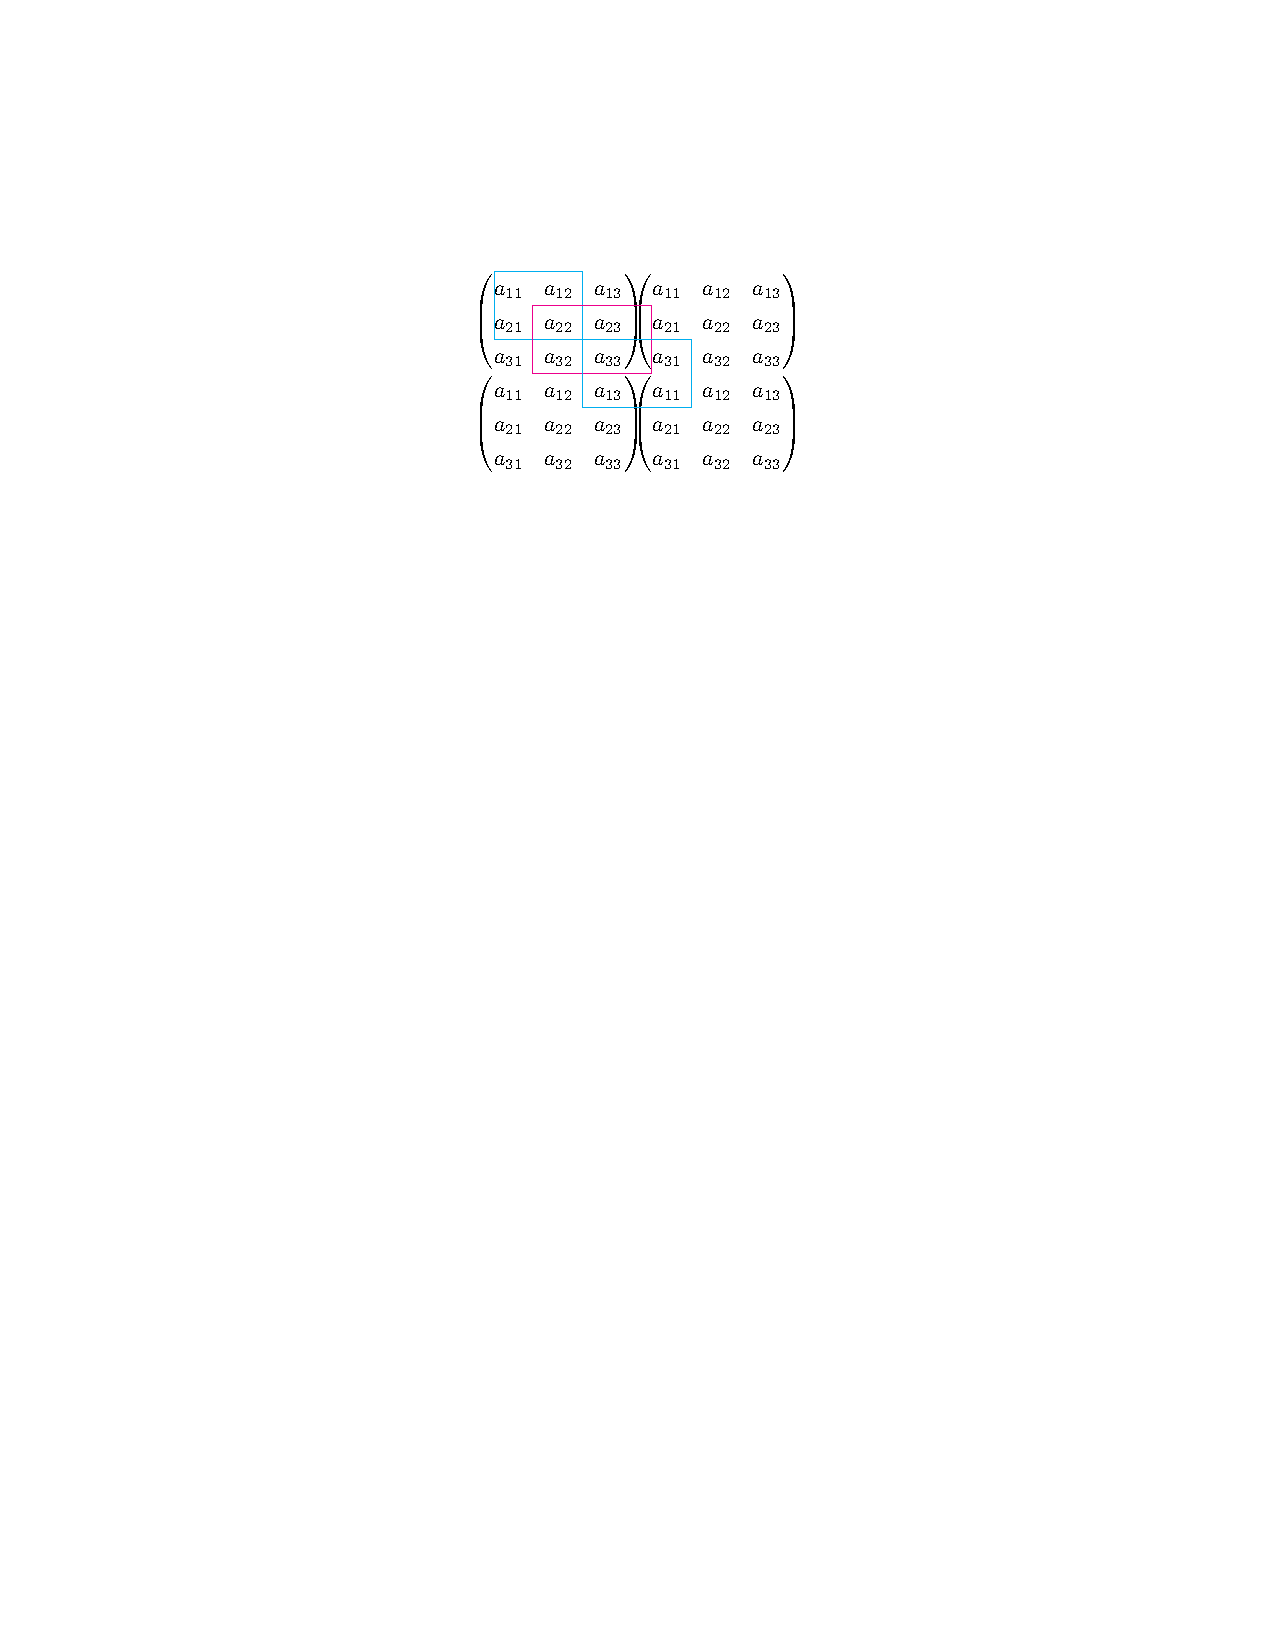
\includegraphics[scale=1]{figures/kjiezzshi.pdf}
    \caption{}
    \label{fig:kjiezzshi}
\end{figure}

\begin{theorem}[特征值的积与和]
    设 $n$ 阶方阵 $\vb*{A}$ 的特征值为 $\lambda_1,\lambda_2,\cdots,\lambda_n$,则 $$\displaystyle\det\vb*{A}=\prod_{i=1}^{n}\lambda_i,~\tr\vb*{A}=\sum_{i=1}^{n}\lambda_i.$$
\end{theorem}

\begin{example}
    设 $\vb*{A}$ 是 3 阶矩阵,$\vb*{A}$ 的特征值为 $1,2,-1$,如果 $\vb*{B}=\vb*{A}^2-2\vb*{A}+3\vb*{E}$,求 $|\vb*{B}|$.
\end{example}
\begin{solution}
    易求得 $\vb*{B}$ 的特征值分别是 $2,3,6$,那么 $\det\vb*{B}=2\times3\times6=36.$
\end{solution}

\begin{theorem}[逆矩阵的特征值]
    矩阵可逆当且仅当其特征值都不等于零,若 $\lambda$ 是可逆矩阵 $\vb*{A}$ 的特征值,则 $\dfrac{1}{\lambda}$ 是逆矩阵 $\vb*{A}^{-1}$ 的特征值.
\end{theorem}

\begin{theorem}[秩一矩阵的特征值]
    若 $n$ 阶方阵 $\vb*{A}$ 满足 $\rank\vb*{A}=1$,那么矩阵 $\vb*{A}$ 的特征值为 $\tr\vb*{A}$ 及 $n-1$ 重 0 根.
\end{theorem}

\begin{example}
    已知 $\vb*{A}$ 是 3 阶矩阵,$\vb*{E}$ 是 3 阶单位矩阵,如果 $\vb*{A},\vb*{A}-2\vb*{E},3\vb*{A}+2\vb*{E}$ 均不可逆,求 $|\vb*{A}+\vb*{E}|.$
\end{example}
\begin{solution}
    易知矩阵 $\vb*{A}$ 的特征值分别为 $0,2,-\dfrac{2}{3}$,那么 $\det(\vb*{A}+\vb*{E})=1\times3\times\dfrac{1}{3}=1.$
\end{solution}

\begin{theorem}[伴随矩阵的特征值 A]
    若 $\vb*{A}$ 为 $n$ 阶可逆矩阵,且 $\lambda_i~ (i=1,2,\cdots,n)$ 是 $\vb*{A}$ 的全部特征值,则 $\dfrac{|\vb*{A}|}{\lambda_i}$ 是 $\vb*{A}^*$ 的全部特征值; 
    若 $\vb*{A}$ 为 $n$ 阶不可逆矩阵,则 $\vb*{A}^*$ 有 $n-1$ 个特征值为 0,另一个特征值为 $\tr\vb*{A}^*.$
\end{theorem}

\begin{theorem}[伴随矩阵的特征值 B]
    \label{bsjzdtzzB}设 $n$ 阶方阵 $\vb*{A}$ 的特征值为 $\lambda_j~ (j=1,2,\cdots,n)$,则 $\vb*{A}^*$ 的 $n$ 个特征值为 $\lambda_i^*$,则
    $$\lambda_i^*=\prod_{\substack{1\leqslant j\leqslant n\\j\neq i}}\lambda_j~  (i=1,2,\cdots,n).$$
\end{theorem}

\begin{example}
    设 $ \vb*{A} $ 为 3 阶矩阵,特征值为 $ \lambda_{1}=\lambda_{2}=1,\lambda_{3}=2 $,
    对应的线性无关的特征向量为 $ \vb*{\alpha}_{1}, \vb*{\alpha}_{2}, \vb*{\alpha}_{3}$,
    令 $ \vb*{P}=\left(\vb*{\alpha}_{1}-\vb*{\alpha}_{3}, \vb*{\alpha}_{2}+\vb*{\alpha}_{3}, \vb*{\alpha}_{3}\right)$,则 $\vb*{P}^{-1} \vb*{A}^{*} \vb*{P}$ 等于
    \begin{tasks}(4)
        \task $\mqty(1&0&0\\0&3&0\\0&0&1)$
        \task $\mqty(-1&0&0\\0&3&0\\0&0&2)$
        \task $\mqty(2&0&1\\0&2&-1\\0&0&1)$
        \task $\mqty(2&0&0\\0&2&0\\1&-1&1)$
    \end{tasks}
\end{example}
\begin{solution}
    由 $\vb*{P}=(\vb*{\alpha}_{1}-\vb*{\alpha}_{3}, \vb*{\alpha}_{2}+\vb*{\alpha}_{3}, \vb*{\alpha}_{3})$,得 $\vb*{P}=(\vb*{\alpha}_1,\vb*{\alpha}_2,\vb*{\alpha}_3)\vb*{E}_{31}(-1)\vb*{E}_{32}(1):=\vb*{B}\vb*{E}_{31}(-1)\vb*{E}_{32}(1)$,那么
    \begin{flalign*}
        \vb*{P}^{-1}\vb*{A}^*\vb*{P}&=(\vb*{B}\vb*{E}_{31}(-1)\vb*{E}_{32}(1))^{-1}\vb*{A}^*\vb*{B}\vb*{E}_{31}(-1)\vb*{E}_{32}(1)=\vb*{E}_{32}(-1)\vb*{E}_{31}(1)\diag(2,2,1)\vb*{E}_{31}(-1)\vb*{E}_{32}(1)\\
        &=\vb*{E}_{32}(-1)\vb*{E}_{31}(1)\vb*{E}_{1}(2)\vb*{E}_{2}(2)\vb*{E}_{31}(-1)\vb*{E}_{32}(1)=\mqty(2&0&0\\0&2&0\\1&-1&1)
    \end{flalign*}
    因此选 D.
\end{solution}

\begin{example}
    已知矩阵 $\vb*{A}=\mqty(1&-1&a\\1&3&5\\0&0&2)$,只有两个线性无关的特征向量,求矩阵 $\vb*{A}$ 的特征值以及 $a$.
\end{example}
\begin{solution}
    由 $|\lambda\vb*{E}-\vb*{A}|=\mqty|\lambda-1&1&-a\\-1&\lambda-3&-5\\0&0&\lambda-2|=(\lambda-1)(\lambda-3)(\lambda-2)+(\lambda-2)=(\lambda-2)^3=0$,于是特征值为 $\lambda_1=\lambda_2=\lambda_3=2$,因为 $n-\rank(2\vb*{E}-\vb*{A})=2$,于是 $\rank(2\vb*{E}-\vb*{A})=1$,进而解得 $a=-5.$
\end{solution}

\begin{theorem}[特征值不等式]
    \label{tzzbds}若 $\vb*{A}$ 的特征值按从小到大排列,即 $\lambda_1\leqslant \lambda_2\leqslant \cdots\leqslant \lambda_n$,则 $$\lambda_1\vb*{x}^\top\vb*{x}\leqslant \vb*{x}^\top\vb*{Ax}\leqslant \lambda_n\vb*{x}^\top\vb*{x}.$$
\end{theorem}
\begin{proof}[{\songti \textbf{证}}]
    存在正交矩阵 $\vb*{Q}$,令 $\vb*{x}=\vb*{Qy}$,使得 $$f(x_1,x_2,\cdots,x_n)=\vb*{x}^\top\vb*{Ax}=\vb*{y}^\top\vb*{Q}^\top\vb*{AQy}=\lambda_1y_1^2+\lambda_2y_2^2+\cdots+\lambda_ny_n^2$$
    不妨设 $\lambda_1\leqslant \lambda_2\leqslant\cdots\leqslant\lambda_n$,有 
    $$\lambda_1\sum_{k=1}^{n}y_k^2\leqslant \sum_{k=1}^{n}\lambda_ky_k^2\leqslant \lambda_n\sum_{k=1}^{n}y_k^2$$
    即 $$\lambda_1\vb*{x}^\top\vb*{x}\leqslant \vb*{x}^\top\vb*{Ax}\leqslant \lambda_n\vb*{x}^\top\vb*{x}.$$
\end{proof}

\begin{theorem}[行均和定理]
    \label{hangjunhedl}若矩阵 $\vb*{A}$ 的每行元素之和均为 $k$,则 $\vb*{A}$ 有一特征值为 $k$,所对应特征向量为 $(1,1,\cdots,1)^\top.$
\end{theorem}

\subsubsection{特征值在求解迭代方程中的应用}

\begin{example}
    给定 3 个数列 $\qty{x_n},\qty{y_n},\qty{z_n}$ 满足 $x_1=-2,y_1=1,z_1=-1$,且当 $n\geqslant 1$ 有
    $$x_{n+1}=3x_n-6y_n-z_n,\quad y_{n+1}=-x_n+2y_n+z_n,\quad z_{n+1}=x_n+3y_n-z_n$$
    求极限 $\displaystyle\lim_{n\to\infty}\dfrac{x_n+y_n+z_n}{3^n+5^n}.$
\end{example}
\begin{solution}
    由 $\begin{cases}
            x_{n+1}=3x_n-6y_n-z_n \\
            y_{n+1}=-x_n+2y_n+z_n \\
            z_{n+1}=x_n+3y_n-z_n
        \end{cases}\Rightarrow \mqty(x_{n+1}\\y_{n+1}\\z_{n+1})=\mqty(3&-6&-1\\-1&2&1\\1&3&-1)\mqty(x_{n}\\y_n\\z_n):=\vb*{A}\mqty(x_{n}\\y_n\\z_n)$,于是特征方程为
    $$\lambda^3-4\lambda^2-7\lambda+10=(\lambda-1)(\lambda-5)(\lambda+2)=0\Rightarrow \lambda_1=1,\lambda_2=5,\lambda_3=-2$$
    于是 $x_n+y_n+z_n=a\cdot 1^n+b\cdot 5^n+c\cdot (-2)^n$,且
    $$\begin{cases}
            x_1+y_1+z_1=-2+1-1=-2=a+5b-2c   \\
            x_2+y_2+z_2=-11+3+3=-6=a+25b+4c \\
            x_3+y_3+z_3=-53+19-4=-38=a+125b-8c
        \end{cases}\Rightarrow \begin{cases}
            a=0             \\
            b=-\dfrac{2}{7} \\[6pt]
            c=\dfrac{2}{7}
        \end{cases}$$
    于是 $x_n+y_n+z_n=-\dfrac{2}{7}\cdot 5^n+\dfrac{2}{7}(-1)^n\cdot 2^n$,那么 $\displaystyle\lim_{n\to\infty}\dfrac{-\dfrac{2}{7}\cdot 5^n+\dfrac{2}{7}(-1)^n\cdot 2^n}{3^n+5^n}=-\dfrac{2}{7}$.
\end{solution}

\subsection{矩阵的特征向量}

\begin{example}
    设矩阵 $\vb*{A}\mqty(3&2&2\\2&3&2\\2&2&3),~\vb*{P}=\mqty(0&1&0\\1&0&1\\0&0&1),~\vb*{B}=\vb*{P}^{-1}\vb*{A}^*\vb*{P}$,求 $\vb*{B}+2\vb*{E}$ 的特征值与特征向量.
\end{example}
\begin{solution}
    设 $\vb*{A}$ 的特征值为 $\lambda$,对应的特征向量为 $\vb*{\xi}$,即 $\vb*{A\xi}=\lambda\vb*{\xi}$,由于 $|\vb*{A}=7\neq0|$,所以 $\lambda\neq0$,于是有 
    $$\vb*{A}^*\vb*{\xi}=\dfrac{|\vb*{A}|}{\lambda}\vb*{\xi},~(\vb*{B}+2\vb*{E})\vb*{P}^{-1}\xi=\qty(\dfrac{|\vb*{A}|}{\lambda}+2)\vb*{P}^{-1}\xi$$
    即 $\dfrac{|\vb*{A}|}{\lambda}+2$ 是 $\vb*{B}+2\vb*{E}$ 的特征值,$\vb*{P}^{-1}\vb*{\xi}$ 为对应的特征向量,
    易求得 $\vb*{A}$ 的特征值为 $\lambda_1=\lambda_2=1,\lambda_3=7$,属于 $\lambda_{1,2}=1$ 的特征向量为 
    $$\vb*{\xi}_1=(-1,1,0)^\top,~\vb*{\xi}_2=(-1,0,1)^\top$$
    属于 $\lambda_3$ 的特征向量为 $\vb*{\xi}_3=(1,1,1)^\top$,因此,$\vb*{B}+2\vb*{E}$ 的三个特征向量为 $9,9,3$,属于特征值 9 的两个线性无关的特征向量为 
    $$\vb*{P}^{-1}\vb*{\xi}_1=(1,-1,0)^\top,~\vb*{P}^{-1}\vb*{\xi}_2=(-1,-1,1)^\top$$
    属于特征值 3 的特征向量为 $\vb*{P}^{-1}\vb*{\xi}_3=(0,1,1)^\top.$
\end{solution}

\begin{example}
    设 $\vb*{A}$ 是线性空间 $\vb*{P}^3$ 的线性变换,已知
    $$\vb*{A}(1,0,0)=(5,6,-3),~\vb*{A}(0,1,0)=(-1,0,1),~\vb*{A}(0,0,1)=(1,2,1)$$
    \begin{enumerate}[label=(\arabic{*})]
        \item 求 $\vb*{A}$ 的全部特征值和特征向量;
        \item 问: 能否找到 $\vb*{P}^3$ 的一组基,使 $\vb*{A}$ 在这组基下的矩阵为对角矩阵?说明理由.
    \end{enumerate}
\end{example}
\begin{solution}
    \begin{enumerate}[label=(\arabic{*})]
        \item $\vb*{A}$ 在基 $(1,0,0),~(0,1,0),~(0,0,1)$ 下的矩阵为
              $\begin{pmatrix}
                      5  & -1 & 1 \\
                      6  & 0  & 2 \\
                      -3 & 1  & 1
                  \end{pmatrix}$,那么 $\vb*{A}$ 的特征多项式为
              $$f(\lambda)=|\lambda\vb*{E}-\vb*{A}|=\begin{vmatrix}
                      \lambda -5 & 1       & -1         \\
                      -6         & \lambda & -2         \\
                      -3         & -1      & \lambda -1
                  \end{vmatrix}\xlongequal[]{}(\lambda-2)^3$$
              所以 $\vb*{A}$ 的特征值为 2,对 $\lambda=2$ 求特征向量,解齐次方程组
              $$\left\{\begin{matrix}
                      -3x_1 & + & x_2  & - & x_3  & =0 \\
                      -6x_1 & + & 2x_2 & - & 2x_3 & =0 \\
                      3x_1  & - & x_2  & + & x_3  & =0
                  \end{matrix}\right.$$
              求得基础解系为: $(1,3,0),~(0,1,1)$,所以 $\vb*{A}$ 的全部特征向量为 $k_1(1,3,0)+k_2(0,1,1)$,其中 $k_1,~k_2$ 为数域 $\vb*{P}$
              中不全为零的任意数,这些特征向量都属于特征值 2.
        \item 因为 $\vb*{A}$ 只有 2 个线性无关的特征向量,而 $\vb*{P}^3$ 是 3 维线性空间,所以找不到一组基,使 $\vb*{A}$ 在这组基下的矩阵为对角矩阵.
    \end{enumerate}
\end{solution}

\begin{example}
    设 $\vb*{A}$ 是线性空间 $\vb*{P}^3$ 的线性变换,
    已知 $$\vb*{A}(1,0,0)=(8,-6,3),~\vb*{A}(1,1,0)=(14,-10,6),~\vb*{A}(1,1,1)=(8,-4,5)$$
    求 $\vb*{A}$ 的全部特征值和特征向量,并求 $\vb*{P}^3$ 的一组基使 $\vb*{A}$ 在这组基下的矩阵为对角矩阵.
\end{example}
\begin{solution}
    因为
    \begin{flalign*}
        \vb*{A}(1,0,0) & =(8,-6,3)=14(1,0,0)-9(1,1,0)+3(1,1,1)    \\
        \vb*{A}(1,1,0) & =(14,-10,6)=24(1,0,0)-16(1,1,0)+6(1,1,1) \\
        \vb*{A}(1,1,1) & =(8,-4,5)=12(1,0,0)-9(1,1,0)+5(1,1,1)
    \end{flalign*}
    所以 $\vb*{A}$ 在基 $(1,0,0),~(1,1,0),~(1,1,1)$ 下的矩阵为
    $\vb*{A}=\begin{pmatrix}
            14 & 24  & 12 \\
            -9 & -16 & -9 \\
            3  & 6   & 5
        \end{pmatrix}$,
    $\vb*{A}$ 的特征多项式为
    $$f(\lambda)=|\lambda \vb*{E}-\vb*{A}|=\begin{vmatrix}
            \lambda -14 & -24         & -12        \\
            9           & \lambda +16 & 9          \\
            -3          & -6          & \lambda -5
        \end{vmatrix}\xlongequal[r_1-4r_3]{r_2+3r_3}\begin{vmatrix}
            \lambda -2 & 0          & -4\lambda +8 \\
            0          & \lambda -2 & 3\lambda -6  \\
            -3         & -6         & \lambda -5
        \end{vmatrix}=(\lambda-2)^2(\lambda+1)$$
    对 $\lambda=-1$ 解齐次方程组
    $$\left\{\begin{matrix}
            -15x_1 & - & 24x_2 & - & 12x_3 & =0 \\
            9x_1   & + & 15x_2 & + & 9x_3  & =0 \\
            -3x_1  & - & 6x_2  & - & 6x_3  & =0
        \end{matrix}\right.$$
    得基础解系: $(4,-3,1)$,对应特征向量为 $4(1,0,0)-3(1,1,0)+(1,1,1)=(2,-2,1)$,所以属于特征值 -1 的全部特征向量为 $k(2,-2,1)$,
    其中 $k$ 为数域 $\vb*{P}$ 中任一非零数;\\
    对 $\lambda=2$ 解齐次方程组
    $$\left\{\begin{matrix}
            -12x_1 & - & 24x_2 & - & 12x_3 & =0 \\
            9x_1   & + & 18x_2 & + & 9x_3  & =0 \\
            -3x_1  & - & 6x_2  & - & 3x_3  & =0
        \end{matrix}\right.$$
        得基础解系 $(-1,0,1),~(0,-1,2)$,对应于特征向量分别为
        $$-(1,0,0)+(1,1,1)=(0,1,1)\text{ 及 }-(1,1,0)+2(1,1,1)=(1,1,2)$$
        所以属于特征值 2 的全部特征向量为 $k_1(0,1,1)+k_2(1,1,2)$,其中 $k_1,~k_2$ 为数域 $\vb*{P}$ 不全为 0 的任意性,
        于是以 $$(2,-2,1),~(0,1,1),~(1,1,2)$$ 为基,则 $\vb*{A}$ 在这组基下的矩阵为对角矩阵 $\mathrm{diag}(-1,2,2).$
\end{solution}

\begin{example}
    设 $\vb*{A}$ 是 3 阶矩阵,$\lambda_1,\lambda_2,\lambda_3$ 是 $\vb*{A}$ 的 3 个不同特征值,对应的特征向量分别为 $\vb*{\alpha}_1,\vb*{\alpha}_2,\vb*{\alpha}_3$,令 $\vb*{\beta}=\vb*{\alpha}_1+\vb*{\alpha}_2+\vb*{\alpha}_3$,
    \begin{enumerate}[label=(\arabic{*})]
        \item 证明: $\vb*{\beta}=\vb*{\alpha}_1+\vb*{\alpha}_2+\vb*{\alpha}_3$ 不是 $\vb*{A}$ 的特征向量;
        \item 证明: $\vb*{\beta},\vb*{A\beta},\vb*{A^2\beta}$ 线性无关;
        \item 若 $\vb*{A}^3\vb*{\beta}=2\vb*{A\beta}$,求 $\vb*{A}$ 的特征值;
        \item 在 (3) 的基础上证明: $\vb*{A\beta}$ 和 $\vb*{A}^2\vb*{\beta}$ 是方程组 $\qty(\vb*{A}^2-2\vb*{E})\vb*{x}=\vb*{0}$ 的基础解系.
    \end{enumerate}
\end{example}
\begin{solution}
    \begin{enumerate}[label=(\arabic{*})]
        \item 反证法: 假设 $\lambda$ 是 $\vb*{A}$ 的特征值,且对应的特征向量为 $\vb*{\beta}$,那么 $\vb*{A\beta}=\lambda\vb*{\beta}$,即
              \begin{flalign*}
                  \vb*{A}(\vb*{\alpha}_1+\vb*{\alpha}_2+\vb*{\alpha}_3)                               & =\lambda(\vb*{\alpha}_1+\vb*{\alpha}_2+\vb*{\alpha}_3)             \\
                  \Rightarrow \vb*{A\alpha}_1+\vb*{A\alpha}_2+\vb*{A\alpha}_3                         & =\lambda\vb*{\alpha}_1+\lambda\vb*{\alpha}_2+\lambda\vb*{\alpha}_3 \\
                  \Rightarrow \lambda_1\vb*{\alpha}_1+\lambda_1\vb*{\alpha}_2+\lambda_1\vb*{\alpha}_3 & =\lambda\vb*{\alpha}_1+\lambda\vb*{\alpha}_2+\lambda\vb*{\alpha}_3 \\
              \end{flalign*}
              即 $\Rightarrow (\lambda_1-\lambda)\vb*{\alpha}_1+(\lambda_2-\lambda)\vb*{\alpha}_2+(\lambda_3-\lambda)\vb*{\alpha}_3=0$,即 $\lambda_1=\lambda_2=\lambda_3$,但这与题意矛盾,故假设不成立,
              即 $\vb*{\beta}=\vb*{\alpha}_1+\vb*{\alpha}_2+\vb*{\alpha}_3$ 不是 $\vb*{A}$ 的特征向量.
        \item 要证: $\vb*{\beta},\vb*{A\beta},\vb*{A^2\beta}$ 线性无关,即证: $k_1\vb*{\beta}+k_2\vb*{A\beta}+k_3\vb*{A}^2\vb*{\beta}=\vb*{0}$,其中 $k_1+k_2+k_3=0$,为此,则有
              $$k_1(\vb*{\alpha}_1+\vb*{\alpha}_2+\vb*{\alpha}_3)+k_2(\lambda_1\vb*{\alpha}_1+\lambda_2\vb*{\alpha}_2+\lambda_3\vb*{\alpha}_3)+k_3\qty(\lambda_1^2\vb*{\alpha}_1+\lambda_2^2\vb*{\alpha}_2+\lambda_3^2\vb*{\alpha}_3)=\vb*{0}$$
              为使等式成立,则有 $$\begin{cases}
                  k_1+k_2\lambda_1+k_3\lambda_1^2=0 \\
                  k_1+k_2\lambda_2+k_3\lambda_2^2=0 \\
                  k_1+k_2\lambda_3+k_3\lambda_3^2=0
              \end{cases}\Rightarrow \mqty|1&\lambda_1&\lambda_1^2\\[6pt]1&\lambda_2&\lambda_2^2\\[6pt]1&\lambda_3&\lambda_3^2|$$
              该行列式为 Vandermonde 行列式,则其值为 $(\lambda_2-\lambda_1)(\lambda_3-\lambda_1)(\lambda_3-\lambda_2)\neq0$,故 $k_1+k_2+k_3=0$,因此 $\vb*{\beta},\vb*{A\beta},\vb*{A^2\beta}$ 线性无关.
        \item 设矩阵 $\vb*{B}\sim\vb*{A}$,且 $\exists\vb*{P}$ 使得 $\vb*{P}^{-1}\vb*{AP}=\vb*{B}$,即 $\vb*{AP}=\vb*{PB}$,不妨取 $\vb*{P}=\qty(\vb*{\beta},\vb*{A\beta},\vb*{A^2\beta})$,因此
              $$\vb*{AP}=\qty(\vb*{A\beta},\vb*{A}^2\vb*{\beta},\vb*{A}^3\vb*{\beta})\xlongequal{\vb*{A}^3\vb*{\beta}=2\vb*{A\beta}}\qty(\vb*{A\beta},\vb*{A}^2\vb*{\beta},2\vb*{A\beta})=\qty(\vb*{\beta},\vb*{A\beta},\vb*{A^2\beta})\mqty(0&0&0\\1&0&2\\0&1&0)$$
              因此 $\vb*{B}=\mqty(0&0&0\\1&0&2\\0&1&0)$,则特征值方程为 $|\lambda\vb*{E}-\vb*{B}|=\mqty|\lambda &0&0\\-1&\lambda&-2\\0&-1&\lambda|=\lambda\mqty|\lambda&-2\\-1&\lambda|=\lambda\qty(\lambda^2-2)=0$,因此特征值为 $\lambda_1=0,\lambda_2=\sqrt{2},\lambda_3=-\sqrt{2}$.
        \item 为证: $\vb*{A\beta}$ 和 $\vb*{A}^2\vb*{\beta}$ 是方程组 $\qty(\vb*{A}^2-2\vb*{E})\vb*{x}=\vb*{0}$ 的基础解系,需分别证:
              \begin{enumerate}[label=(\roman{*})]
                  \item $\vb*{A\beta}$ 和 $\vb*{A}^2\vb*{\beta}$ 是方程组 $\qty(\vb*{A}^2-2\vb*{E})\vb*{x}=\vb*{0}$ 的解;\\
                        当 $\vb*{x}=\vb*{A\beta}$ 时,有 $\qty(\vb*{A}^2-2\vb*{E})\vb*{A\beta}=\vb*{A}^3\vb*{\beta}-2\vb*{A\beta}\xlongequal{\vb*{A}^3\vb*{\beta}=2\vb*{A\beta}}\vb*{0}$ 成立;\\
                        当 $\vb*{x}=\vb*{A}^2\vb*{\beta}$ 时,有 $\qty(\vb*{A}^2-2\vb*{E})\vb*{A}^2\vb*{\beta}=\vb*{A}^4\vb*{\beta}-2\vb*{A}^2\vb*{\beta}=\vb*{A}\qty(\vb*{A}^3\vb*{\beta}-2\vb*{A\beta})\xlongequal{\vb*{A}^3\vb*{\beta}=2\vb*{A\beta}}\vb*{0}$ 成立;
                  \item $\vb*{A\beta}$ 和 $\vb*{A}^2\vb*{\beta}$ 线性无关;\\
                        由 (2) 可知 $\vb*{\beta},\vb*{A\beta},\vb*{A^2\beta}$ 线性无关 \textcolor{red}{(整体无关,部分必无关; 部分相关,整体必相关)},故 $\vb*{A\beta}$ 和 $\vb*{A}^2\vb*{\beta}$ 线性无关;
                  \item $S=n-\rank\qty(\vb*{A}^2-2\vb*{E})$,其中 $S=2$.\\
                        因为 $\vb*{P}^{-1}\vb*{AP}=\vb*{\Lambda}_1$,即 $\vb*{A}$ 能相似对角化,故 $\vb*{P}^{-1}\qty(\vb*{A}^2-2\vb*{E})\vb*{P}$ 亦能相似对角化为矩阵 $\vb*{\Lambda}_2$,又因为 $\qty(\vb*{A}^2-2\vb*{E})$ 的特征值为 $2,0,0$,那么 $\rank\qty(\vb*{A}^2-2\vb*{E})=1$,且 $n=3$,故 $S=n-\rank\qty(\vb*{A}^2-2\vb*{E})$ 成立,
              \end{enumerate}
              综上所述,$\vb*{A\beta}$ 和 $\vb*{A}^2\vb*{\beta}$ 是方程组 $\qty(\vb*{A}^2-2\vb*{E})\vb*{x}=\vb*{0}$ 的基础解系.
    \end{enumerate}
\end{solution}

\subsection{公共特征向量}

\begin{theorem}[方阵的公共特征向量]
    若 $n$ 阶方阵 $\vb*{A},~\vb*{B}$ 满足 $\vb*{AB}=\vb*{BA}$,则 $\vb*{A}$ 与 $\vb*{B}$ 一定有公共的特征向量.
\end{theorem}

\subsection{Schmidt 正交化}

\begin{theorem}[Schmidt 正交化]
    设向量组 $ \vb*{\alpha}_{1}, \vb*{\alpha}_{2}, \cdots, \vb*{\alpha}_{n} $ 线性无关,则必存在正交组
    $\vb*{\beta}_{1}, \vb*{\beta}_{2}, \cdots, \vb*{\beta}_{n}$,使得 $ \vb*{\beta}_{i} $ 可由向量组
    $\vb*{\alpha}_{1}, \vb*{\alpha}_{2}, \cdots, \vb*{\alpha}_{n} $ 线性表出,其表出公式如下:
    \begin{flalign*}
        \vb*{\beta}_{1} & =\vb*{\alpha}_{1},                                                                                                                                                                                                                                                                                                                                                                              \\
        \vb*{\beta}_{2} & =\vb*{\alpha}_{2}-\frac{\left[\vb*{\alpha}_{2}, \vb*{\beta}_{1}\right]}{\left[\vb*{\beta}_{1}, \vb*{\beta}_{1}\right]} \vb*{\beta}_{1}                                                                                                                                                                                                                                                          \\
        \vdots          &                                                                                                                                                                                                                                                                                                                                                                                                 \\
        \vb*{\beta}_{n} & =\vb*{\alpha}_{n}-\frac{\left[\vb*{\alpha}_{n}, \vb*{\beta}_{1}\right]}{\left[\vb*{\beta}_{1}, \vb*{\beta}_{1}\right]} \vb*{\beta}_{1}-\frac{\left[\vb*{\alpha}_{n}, \vb*{\beta}_{2}\right]}{\left[\vb*{\beta}_{2}, \vb*{\beta}_{2}\right]} \vb*{\beta}_{2}-\cdots -\frac{\left[\vb*{\alpha}_{n}, \vb*{\beta}_{n-1}\right]}{\left[\vb*{\beta}_{n-1}, \vb*{\beta}_{n-1}\right]} \vb*{\beta}_{n-1}
    \end{flalign*}
    若再把正交向量组 $ \vb*{\beta}_{1}, \vb*{\beta}_{2} \cdots \vb*{\beta}_{n} $ 单位化,即令
    $$\vb*{e}_{1}=\frac{\vb*{\beta}_{1}}{\left\|\vb*{\beta}_{1}\right\|}, \vb*{e}_{2}=\frac{\vb*{\beta}_{2}}{\left\|\vb*{\beta}_{2}\right\|}, \cdots, \vb*{e}_{n}=\frac{\vb*{\beta}_{n}}{\left\|\vb*{\beta}_{n}\right\|},$$
    则 $ \vb*{e}_{1}, \vb*{e}_{2}, \cdots, \vb*{e}_{n} $ 是标准正交向量组.
\end{theorem}

\begin{example}[2021 数一]
    已知 $\vb*{\alpha}=\mqty(1\\0\\1),~\vb*{\alpha}_2=\mqty(1\\2\\1),~\vb*{\alpha}=\mqty(3\\1\\2)$,记 $\vb*{\beta}_1=\vb*{\alpha}_1,~\vb*{\beta}_2=\vb*{\alpha}_2-k\vb*{\beta}_1,~\vb*{\beta}_3=\vb*{\alpha}_3-l_1\vb*{\beta}_1-l_2\vb*{\beta}_2$,
    若 $\vb*{\beta}_1,\vb*{\beta}_2,\vb*{\beta}_3$ 两两正交,则 $l_1,~l_2$ 依次为
    \begin{tasks}(4)
        \task $\dfrac{5}{2},~\dfrac{1}{2}$
        \task $-\dfrac{5}{2},~\dfrac{1}{2}$
        \task $\dfrac{5}{2},~-\dfrac{1}{2}$
        \task $-\dfrac{5}{2},~-\dfrac{1}{2}$
    \end{tasks}
\end{example}
\begin{solution}
    \textbf{法一: }因为 $\vb*{\beta}_1$ 与 $\vb*{\beta}_2$ 相互正交,即 $$(1,0,1)\cdot(1-k,2,1-k)=0\Rightarrow k=1\Rightarrow \vb*{\beta}_2=\vb*{\alpha}_2-\vb*{\beta}_1$$
    同理 $\vb*{\beta}_1$ 与 $\vb*{\beta}_3$ 相互正交,$\vb*{\beta}_2$ 与 $\vb*{\beta}_3$ 相互正交,则 
    $$\begin{cases}
        (1,0,1)\cdot(3-l_1,1-2l_2,2-l_1)=0\\
        (0,2,0)\cdot(3-l_1,1-2l_2,2-l_1)=0
    \end{cases}\Rightarrow \begin{cases}
        l_1=\dfrac{5}{2}\\[6pt]
        l_2=\dfrac{1}{2}
    \end{cases}$$
    \textbf{法二: }$\vb*{\beta}_2=\vb*{\alpha}_2-\dfrac{[\vb*{\alpha}_2,\vb*{\beta}_1]}{[\vb*{\beta}_1,\vb*{\beta}_1]}\vb*{\beta}_1=\mqty(0\\2\\0),~\vb*{\beta}_3=\vb*{\alpha}_3-\dfrac{[\vb*{\alpha}_3,\vb*{\beta}_2]}{[\vb*{\beta}_2,\vb*{\beta}_2]}\vb*{\beta}_2-\dfrac{[\vb*{\alpha}_3,\vb*{\beta}_1]}{[\vb*{\beta}_1,\vb*{\beta}_1]}\vb*{\beta}_1$,
    因此 $l_1=\dfrac{[\vb*{\alpha}_3,\vb*{\beta}_1]}{[\vb*{\beta}_1,\vb*{\beta}_1]}=\dfrac{5}{2},~l_2=\dfrac{[\vb*{\alpha}_3,\vb*{\beta}_2]}{[\vb*{\beta}_2,\vb*{\beta}_2]}=\dfrac{1}{2}$,
    故选 A.
\end{solution}
